\chapter{Adaptacyjne metody eliminacji zakłóceń}
\section{Algorytm najmniejszych kwadratów}
Algorytm najmniejszych kwadratów (LMS od ang. \textit{Least Mean Squares}) działa dwuetapowo.
\begin{enumerate}
\item Etap filtracji, na który składa się obliczenie wyjścia filtru o pewnej długości i współczynnikach (odczepach) oraz estymacja sygnału błędu będąca różnicą pomiędzy wyjściem filtra a pożądaną odpowiedzią.
\item Etap adaptacji, który powoduje dostosowanie się współczynników filtra na podstawie sygnału błędu.
\end{enumerate}
Na rys. \ref{lms_filter} przedstawiono przepływ sygnałów w strukturze filtra. 
Dla danego ciągu wejściowego $x(n)$ filtr produkuje sygnał wyjściowy $\hat{y}(n)$, który jest porównywany do sygnału pożądanego $d(n)$. 
Błąd estymacji $e(n)$ jest różnicą pomiędzy sygnałem pożądanym a jego estymacją $\hat{y}(n)$. 
Sygnał błędu zamyka pętlę sprzężenia zwrotnego. \cite{Haykin:1996:AFT:230061} 
Adaptacja może zostać osiągnięta przez obserwację błędu między pożądanym a rzeczywistym kształtem impulsów mierzonych na wyjściu filtru w chwilach próbkowania i posłużenie się tym błędem do wyznaczania kierunków zmian w wagach odczepów. \cite{Haykin:1998:ST}

\begin{figure}[ht]
\centering
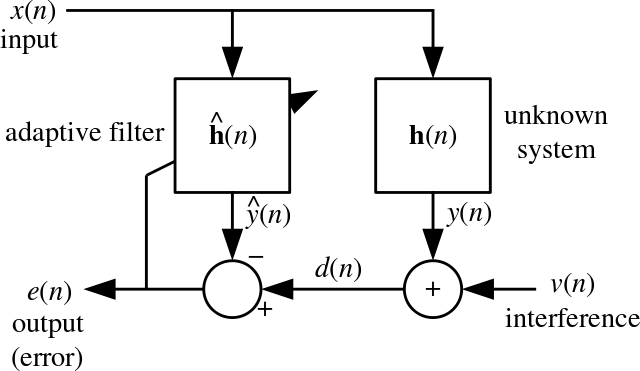
\includegraphics[scale=0.5]{ch6_lms_diagram.png}
\caption[Schemat budowy filtra adaptacyjnego.; Źródło: \textit{https://en.wikipedia.org/wiki/Least_mean_squares_filter}]{\tabular[t]{@{}l@{}}Schemat budowy filtra adaptacyjnego. \\ Źródło: \textit{https://en.wikipedia.org/wiki/Least\_mean\_squares\_filter}\endtabular}
\label{lms_filter}
\end{figure}

Wzór opisujący zmiany współczynników wag odczepów wyraża się w następujący sposób:
\begin{equation}
\hat{w}_k(n+1) = \hat{w}_k(n) + \mu e_nx_{n-k}, \quad k= 0,1...,N
\end{equation}
Tutaj $\hat{w}_k(n+1)$ jest skorygowaną o $\mu e_nx_{n-k}$ wartością współczynnika $\hat{w}_k(n)$. 
Niewielka stała dodatnie $\mu$ nazywana jest parametrem stopniowania. \cite{Haykin:1998:ST} 

Aby podkreślić zespoloną naturę algorytmu używa się notacji z rozbiciem na sygnały kwadraturowe:
\begin{itemize}
\item Wyjście filtra:
\begin{equation} \label{eq:yn}
y(n) = \bm{\hat{w}}^H(n) \bm{x}(n)
\end{equation}
\begin{equation}
y_I(n) = \bm{\hat{w}}_I^T(n) \bm{x}_I(n) - \bm{\hat{w}}_Q^T(n) \bm{x}_Q(n)
\end{equation}
\begin{equation}
y_Q(n) = \bm{\hat{w}}_I^T(n) \bm{x}_Q(n) - \bm{\hat{w}}_Q^T(n) \bm{x}_I(n)
\end{equation}
\item Błąd estymacji:
\begin{equation}
e(n) = d(n) - y(n)
\end{equation}
\begin{equation}
e_I(n) = d_I(n) - y_I(n)
\end{equation}
\begin{equation}
e_Q(n) = d_Q(n) - y_Q(n)
\end{equation}
\item Wektor wag odczepów
\begin{equation}
\bm{\hat{w}}(n+1) = \bm{\hat{w}}(n) + \mu \bm{x}(n)e^*(n)
\end{equation}
\begin{equation}
\bm{\hat{w}_I}(n+1) = \bm{\hat{w}_I}(n) + \mu [e_I(n) \bm{x}_I(n) - e_Q(n) \bm{x}_Q(n)]
\end{equation}
\begin{equation}
\bm{\hat{w}_Q}(n+1) = \bm{\hat{w}_Q}(n) + \mu [e_I(n) \bm{x}_Q(n) - e_Q(n) \bm{x}_I(n)]
\end{equation}
\end{itemize}

\section{Korekcja adaptacyjna}

Korektor działa w oparciu o filtr adaptacyjny i kryterium najmniejszych kwadratów.
Rysunek \ref{fig:eq} przedstawia konstrukcję korektora.
Sygnał pierwszego generatora losowego $x_n$ jest wejściem układu i służy do testowania kanału, natomiast sygnał $v(n)$ generowany przez drugie źródło losowe, wprowadza do układu addytywny szum biały. 
Korektor ma za zadanie zlikwidować szum obecny w kanale poprzez adaptacyjną filtrację.

\begin{figure}[ht]
\centering
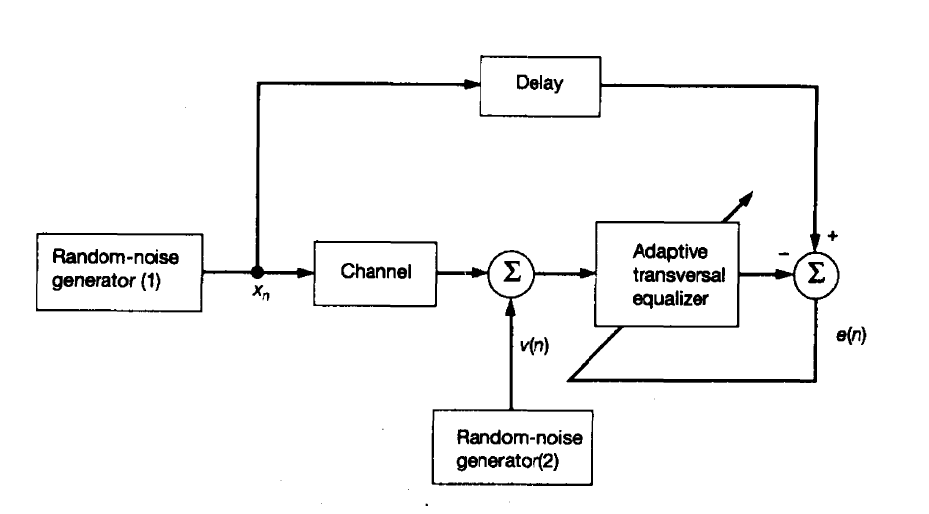
\includegraphics[scale=0.65]{ch6_eq}
\caption{Schemat korektora adaptacyjnego}
\label{fig:eq}
\end{figure}
